\documentclass[twoside]{article}
\usepackage{amsgen,amsmath,amstext,amsbsy,amsopn,amssymb,hyperref}
\usepackage{graphicx}
\usepackage{epsfig}

\setlength{\oddsidemargin}{0.1 in} \setlength{\evensidemargin}{-0.1
in} \setlength{\topmargin}{-0.6 in} \setlength{\textwidth}{6.5 in}
\setlength{\textheight}{10.4 in} \setlength{\headsep}{0.1 in}
\setlength{\parindent}{0 in} \setlength{\parskip}{0.1 in}

\newcommand{\homework}[2]{
   \pagestyle{myheadings}
   \thispagestyle{plain}
   \newpage
   \setcounter{page}{1}
   \noindent
   \begin{center}
   \framebox{
      \vbox{\vspace{2mm}
       \hbox to 6.28in { {\bf Math 1700:~Elementary Statistics \hfill} }
       \vspace{6mm}
       \hbox to 6.28in { {\Large \hfill #1 (#2)  \hfill} }
       \vspace{6mm}
      \vspace{2mm}}
   }
   \end{center}
   \markboth{#1}{#1}
   \vspace*{4mm}
}

\newcommand{\bbF}{\mathbb{F}}
\newcommand{\bbX}{\mathbb{X}}
\newcommand{\bI}{\mathbf{I}}
\newcommand{\bX}{\mathbf{X}}
\newcommand{\bY}{\mathbf{Y}}
\newcommand{\bepsilon}{\boldsymbol{\epsilon}}
\newcommand{\balpha}{\boldsymbol{\alpha}}
\newcommand{\bbeta}{\boldsymbol{\beta}}
\newcommand{\0}{\mathbf{0}}

\begin{document}

\homework{$7^{th}$ and $8^{th}$ Weeks Summary}{10/16/25}
\vspace{-.3in}
\begin{itemize}
\item Inference about the value of the population mean, $\mu$.
\item Estimating the value of a population parameter ($\mu$).
\subitem Point estimate for a parameter ($\bar{x}$)
\subitem Interval estimate ($\bar{x} - E$, $\bar{x} + E$)
\item Level of confidence $(1-\alpha)$: The portion of all interval estimates that include the parameter being estimated.
\item Confidence interval for $\mu$: An interval estimate with a specified level $(1–\alpha)$ of confidence:
\subitem $(\bar{x}-z(\alpha/2)\dfrac{\sigma}{\sqrt{n}}, \bar{x}+z(\alpha/2)\dfrac{\sigma}{\sqrt{n}})$
\subitem Maximum error of Estimate: $E=z(\alpha/2)\biggl(\dfrac{\sigma}{\sqrt{n}}\biggr)$
\subitem \href{https://www.statcrunch.com/applets/type3&cimean}{Confidence Interval Applet}
\item Required Sample size for a specific level of confidence, $(1-\alpha)$:
\subitem $n=\biggl(\dfrac{z(\alpha/2)\sigma}{E}\biggr)^2$
\item Testing a hypothesis.\dotfill
\subitem Null Hypothesis: 
\subsubitem $H_0: \mu = \mu_0$
\subitem Alternative (Research) Hypotheses: 
\subsubitem $H_a: \mu < \mu_0$, or
\subsubitem $H_a: \mu > \mu_0$, or
\subsubitem $H_a: \mu \neq \mu_0$
\item Type of Errors:
\subitem Type I Error or Level of Significance $(\alpha)$: 
\subsubitem Falsely Rejecting $H_0$
\subitem Type II Error $(\beta)$: 
\subsubitem Falsely Fail to Reject $H_0$
\item Test Statistic:
\subitem $z^*=\dfrac{\bar{x}-\mu_0}{\sigma/\sqrt{n}}$
\item Hypothesis Test Approaches
\subitem Classical Approach
\subitem P-value Approach
\item P-value Approach HT: A 5-step Procedure
\subitem Step 1 The Set-Up
\subitem Step 2 The Hypothesis Test Criteria
\subitem Step 3 The Sample Evidence
\subitem Step 4 The Probability Distribution
\subitem Step 5 The Results
\end{itemize}
\vspace{-5.6in}\begin{figure}[h]
\hspace{3.2in}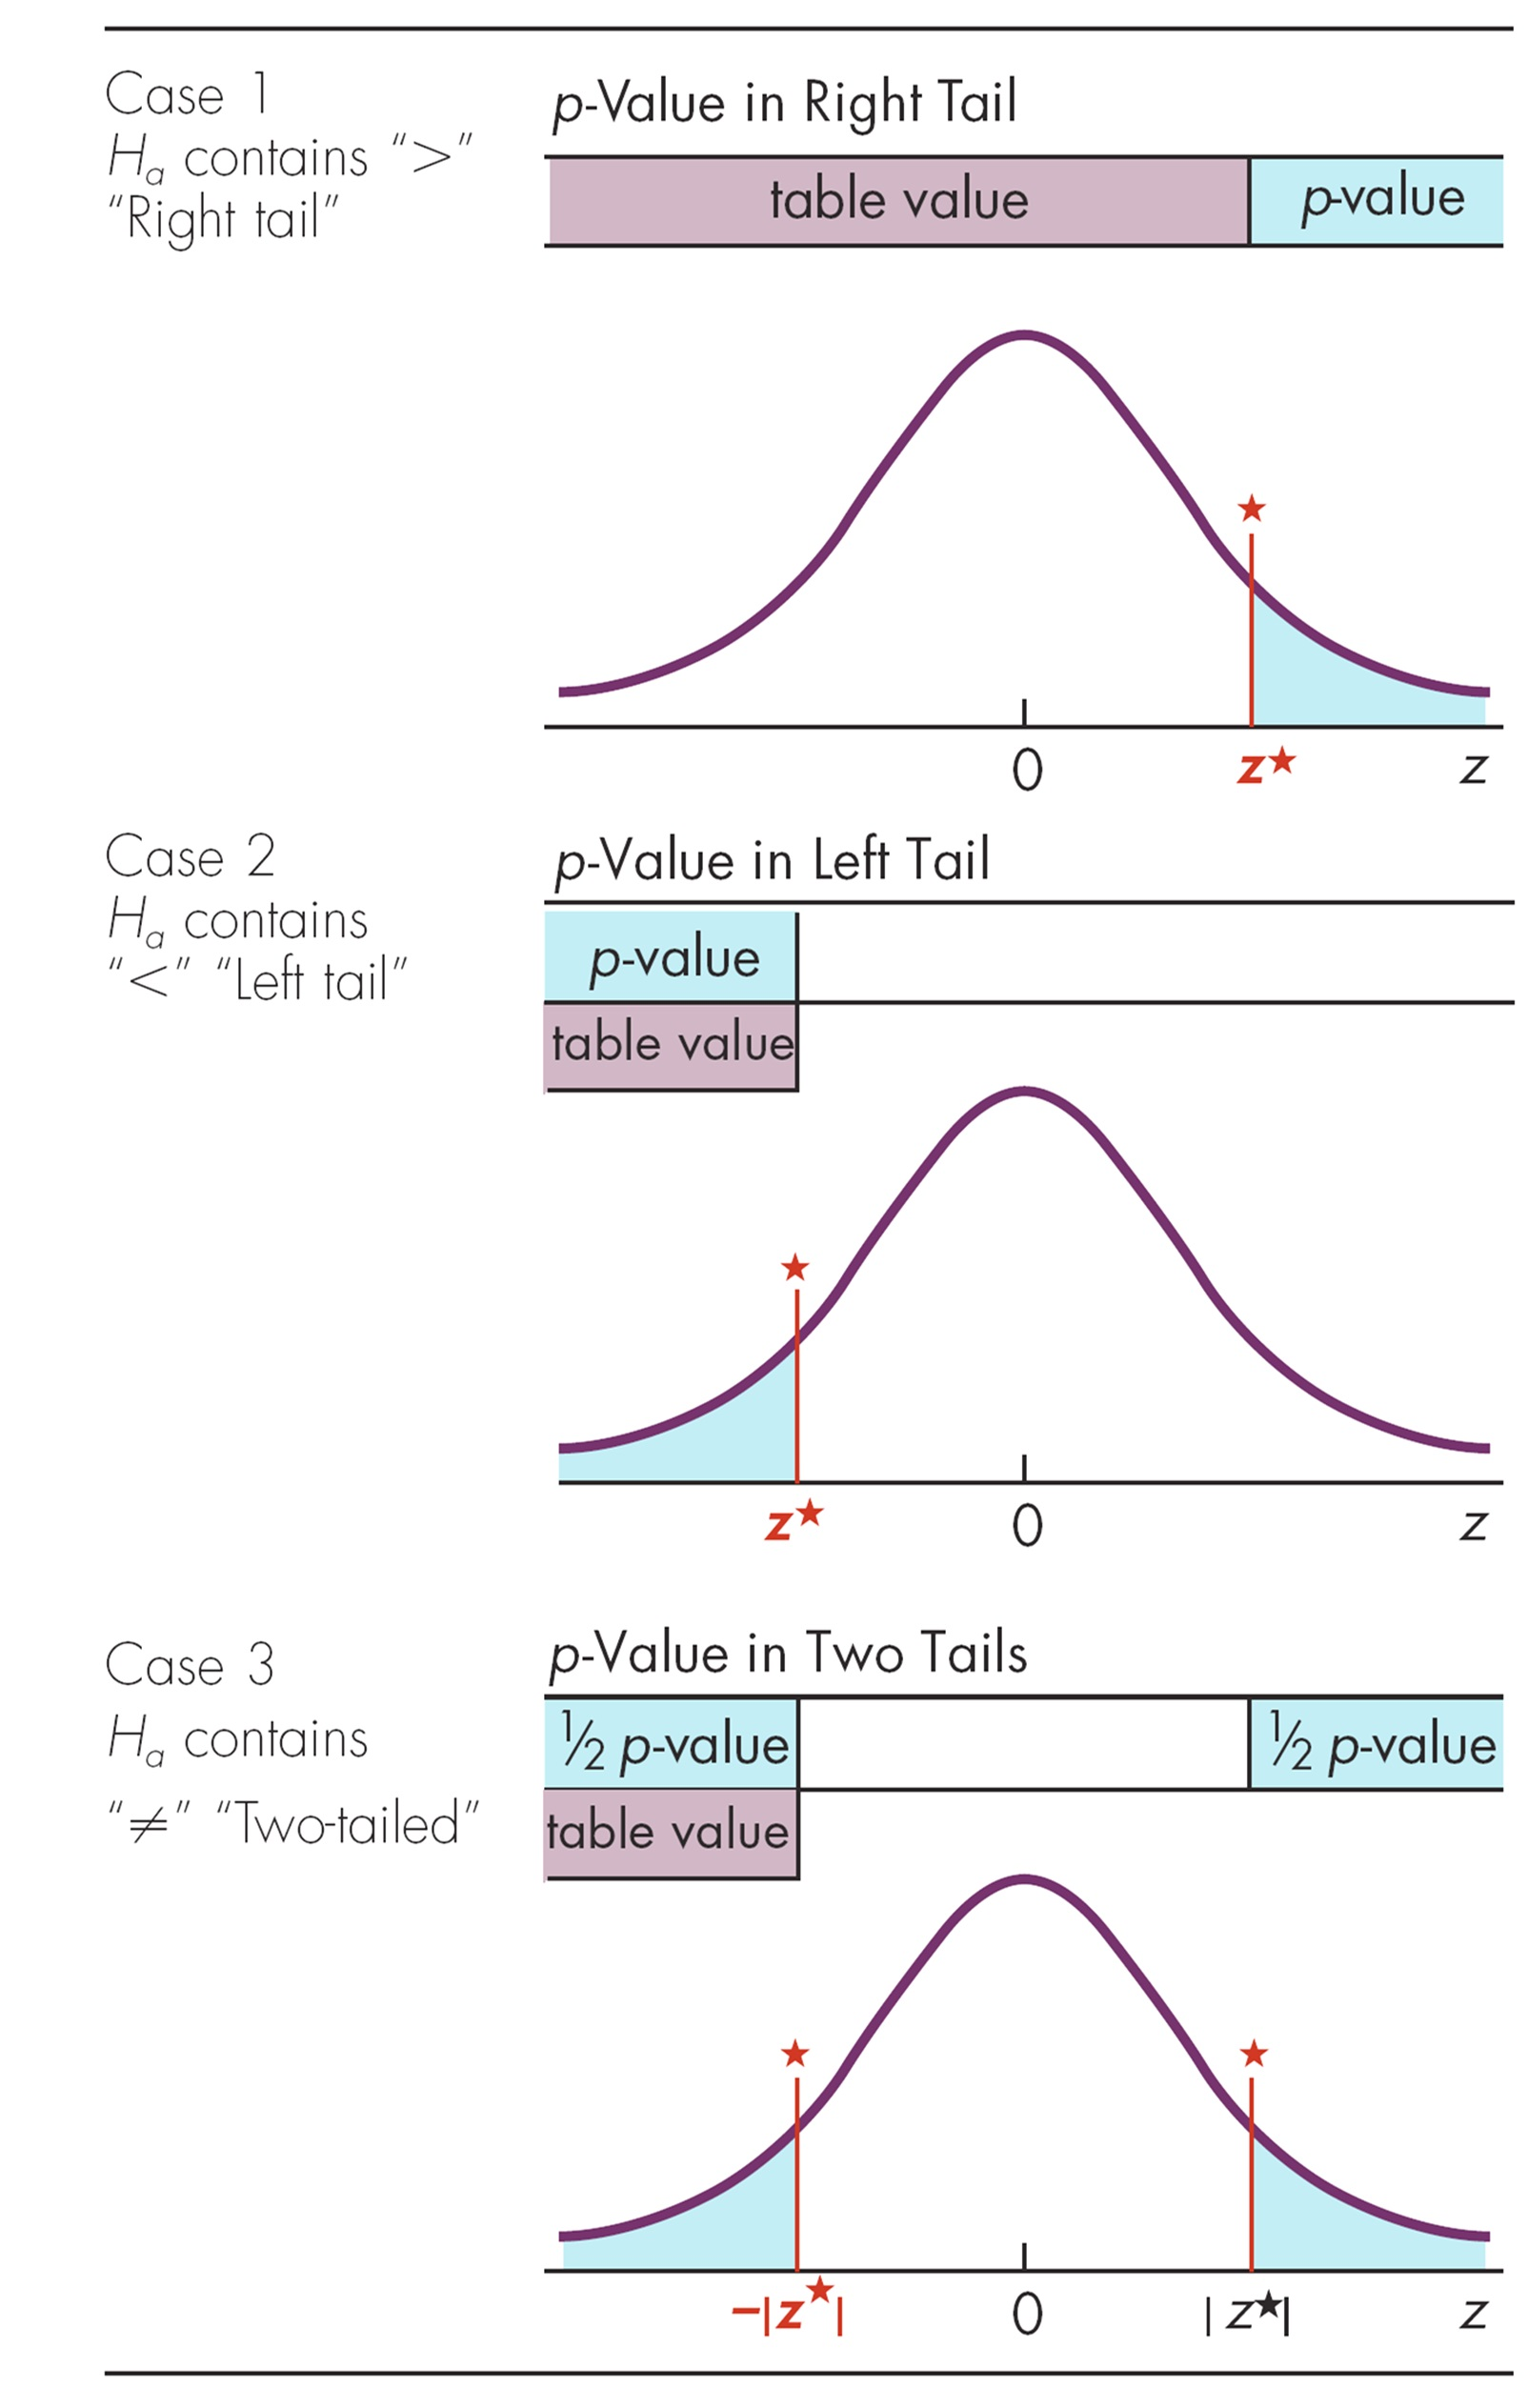
\includegraphics[angle=0,width=.55\textwidth] {graphs9.jpg}
\end{figure}
\newpage
\begin{itemize}
\item Classical approach of Hypothesis Testing\dotfill
\begin{figure}[h]
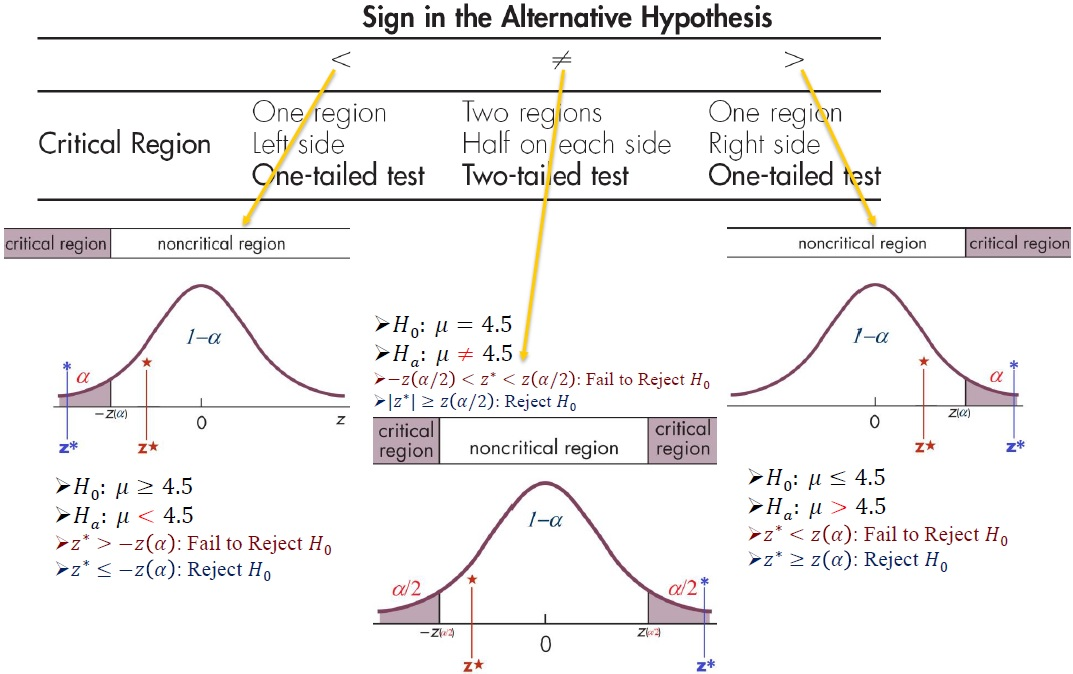
\includegraphics[angle=0,width=\textwidth] {graphs10.jpg}
\end{figure}
\end{itemize}
\end{document}
